% se puede agregar la opción [english] para 
%  memorias o tesis en inglés (borrando el archivo .aux)
\documentclass[hyphens]{umemoria} 
%\includeonly{teorico}
\depto{Departamento de Física}
\author{Diego Antonio Román Cortés}
\title{Acoplamientos no convencionales y transiciones topológicas en sistemas fotónicos multiorbitales}

% incluir ambos comandos para una doble titulación
%  o quitar el comando que no aplica
%\memoria{Ingenier[o/a?] Civil en ???}
\tesis{Magíster en, Ciencias, mención Física}
%\tesis{Doctor en ???} % incluir solo este comando para doctorados

% puede haber varios profesores guía seperados por coma;
% pero si es una memoria, solo puede haber un profesor guía
\guia{Rodrigo Andrés Vicencio Poblete} 

% puede haber varios profesores co-guía seperados por coma;
% pero si es una memoria, el profesor co-guía será el primer
% integrante de la comisión
%\coguia{Nombre Completo Co-Guía} % incluir en caso de co-guía de *tesis*

%\cotutela{Nombre Institución} % incluir en caso de cotutela

\comision{Carla Hermann Avigliano, Pedro Orellana}

\auspicio{los proyectos Instituto Milenio para la Investigación en Óptica (MIRO) ICN17$\_$012 y Fondecyt Regular 1231313 \\ Powered@NLHPC: Esta tesis fue parcialmente apoyada por la infraestructura de supercómputo del NLHPC (CCSS210001)} % incluir en caso de recibir financiamiento

% tiene que ser el año en que se da el examen de título/grado (defensa)
%\anho{2021} % incluir solo para reemplazar el año actual

\usepackage{amsmath, bm}
\usepackage{bm}
\usepackage{lipsum}
\usepackage{pgfplots}
\usepackage{txfonts}
\usepackage{graphicx}
%\usepackage[spanish, es-nodecimaldot]{babel}
\usepackage{float}
\usepackage[figurename=Figura]{caption}
\usepackage[numbers, sort&compress]{natbib}
%\usepackage[hyphens]{url}
\usepackage{indentfirst}
\usepackage{hyperref}
\usepackage{xcolor}
\usepackage{ragged2e}
\usepackage{cancel}
\usepackage[rightcaption]{sidecap}
\usepackage{titlesec}
\usepackage{listings}
\usepackage{mathtools}
\usepackage{xcolor}
\usepackage{setspace}
\usepackage{parskip}
\usepackage{fontspec} % Necesario para fuentes específicas
\usepackage{titlesec}
\usepackage{etoolbox}
\usepackage{alphalph}
\usepackage{chngcntr}

\definecolor{codegreen}{rgb}{0,0.6,0}
\definecolor{codegray}{rgb}{0.5,0.5,0.5}
\definecolor{codepurple}{rgb}{0.58,0,0.82}
\definecolor{backcolour}{rgb}{0.95,0.95,0.92}

\lstdefinestyle{mystyle}{
    backgroundcolor=\color{backcolour},   
    commentstyle=\color{codegreen},
    keywordstyle=\color{magenta},
    numberstyle=\tiny\color{codegray},
    stringstyle=\color{codepurple},
    basicstyle=\ttfamily\footnotesize,
    breakatwhitespace=false,         
    breaklines=true,                 
    captionpos=b,                    
    keepspaces=true,                 
    numbers=left,                    
    numbersep=5pt,                  
    showspaces=false,                
    showstringspaces=false,
    showtabs=false,                  
    tabsize=2
}

\lstset{style=mystyle}

\begin{document}

\frontmatter
\maketitle

\begin{resumen}\ignorespacesafterend
	En esta tesis se estudian fenómenos de acoplamiento no convencionales en redes fotónicas multiorbitales, fabricadas mediante la técnica de escritura por láser de femtosegundos. Se investigan mecanismos que trascienden el acoplamiento entre modos fundamentales, incorporando grados de libertad orbitales, asimetrías estructurales y efectos topológicos. La propagación de luz se analiza en configuraciones donde los modos transversales \( S \) y \( P \) interactúan de manera controlada, revelando nuevas formas de manipulación óptica basadas en simetría, geometría y estructura modal.
	
	En primer lugar, se investiga el fenómeno de \textit{invisibilidad dipolar} de los modos dipolares \( P \), demostrando experimentalmente que, bajo ciertas condiciones geométricas, estos pueden permanecer ópticamente desacoplados. Este efecto se observa en una red fotónica tipo grafeno  y se modela teóricamente mediante una extensión de la teoría de modos acoplados que incorpora tanto acoplamientos de largo alcance como no ortogonalidad entre modos.
	
	Luego, se estudia el fenómeno de \textit{acoplamiento evanescente no simétrico} en dímeros con diferentes contrastes de índice de refracción. Se presenta una formulación generalizada de la teoría de modos acoplados que da cuenta de esta asimetría inherente, incluso en ausencia de pérdida o ganancia. Se valida experimentalmente la ruptura de reciprocidad mediante mediciones de desbalance de intensidad dependientes del canal de entrada.
	
	Posteriormente, se explora el \textit{acoplamiento interorbital \( S\hspace{-0.3ex}P \)}, un mecanismo que permite hibridar modos de simetría transversal distinta mediante la sintonización precisa de sus constantes de propagación. A partir de esta técnica, se implementa una red que realiza el modelo SP-SSH, una extensión multiorbital del modelo de Su-Schrieffer-Heeger. Este sistema presenta una doble transición de fase topológica, determinada por la dimerización geométrica y el desintonizado orbital, que da lugar a tres fases distintas caracterizadas mediante polarización de bulto y análisis espectral.
	
	Los resultados experimentales y numéricos presentados en esta tesis revelan nuevas formas de controlar la propagación de luz utilizando los grados de libertad orbitales de los modos guiados, abriendo el camino hacia el diseño de redes fotónicas avanzadas con funcionalidad topológica y direccional.
\end{resumen}

% opcional: incluir para tesis en inglés;
%  en este caso hay que tener el resumen y abstract
%   en ambos idiomas
%\begin{abstract}
%\lipsum[1-4]
%\end{abstract}

\begin{dedicatoria}


Mas si buscáis descubrimientos\\
Tierras irrealizables más allá de los cielos\\
Vegetante obsesión de musical congoja\\
Volvamos al silencio\\
Trampas de luz y cascadas lujosas\\
Trampas de perla y de lámpara acuática\\
Anda como los ciegos con sus ojos de piedra\\
Presintiendo el abismo a todo paso\\
Mas no temas de mí que mi lenguaje es otro\\
No trato de hacer feliz ni desgraciado a nadie\\
Ni descolgar banderas de los pechos\\
Ni dar anillos de planetas\\
Ni hacer satélites de mármol en torno a un talismán ajeno\\
Quiero darte una música de espíritu\\
Música mía de esta cítara plantada en mi cuerpo\\
Música que hace pensar en el crecimiento de los árboles\\
Y estalla en luminarias dentro del sueño\\
\textnormal{\\Extractos de \textit{Altazor}, Vicente Huidobro}
\end{dedicatoria}

\begin{thanks}
Detrás de cada logro hay una constelación de personas que lo hicieron posible. Aunque sea imposible nombrarlas a todas, guardo en mi memoria el agradecimiento profundo por sus enseñanzas, su tiempo y su confianza. \\

En primer lugar, a mi círculo más íntimo:
\begin{itemize}
\item A mis padres, por sus enseñanzas, valores y experiencias que llevaré siempre conmigo.
\item A mi hermano Martín, por las incontables noches de animé, juegos y cómplices risas.
\item A mi pareja, Catalina, por su apoyo incondicional y cariño en los momentos más sombríos, y por ser mi refugio y motivación en los más brillantes.
\end{itemize}
Agradezco a Pablo y a Cristóbal, mis pilares desde ya catorce años: por las tonterías que superan a las seriedades, por los silencios cómodos y las juntas espontáneas que parecen no tener fin. 

Un agradecimiento especial a los insufribles \textit{Amazing} Fabián y \textit{Amazing} Carlos, por hacer los días de trabajo más llevaderos y por escucharme cuando más lo necesité, por empujarme cuando más lo necesitaba y por motivarme a sacar lo mejor de mí incluso cuando no creía en ello.

Un lugar muy particular lo tienen los integrantes —pasados, presentes y futuros— del Grupo de Redes Fotónicas:
\begin{itemize}
\item A Rodrigo, por acoger hace cinco años al entonces \textit{mechón} de Licenciatura en Física que era, por confiar en mí y enseñarme todo lo que sé sobre Redes Fotónicas, acercarme al mundo académico y darme lecciones de vida que cargaré como brújula hacia el futuro.
\item A Paloma, Bastián, Ignacio y Diego, por su infinita paciencia, su ayuda desinteresada y por hacer de cada jornada en el laboratorio que estuve con ellos un espacio de aprendizaje, colaboración y camaradería que atesoraré siempre.
\item A Polette, Romina, Lucas, Daniel y Sofía, por otorgarle colores cálidos y vibrantes al LABGO3, por ser los mejores colegas que pude haber tenido y por las risas, los buenos chismes y el aprendizaje constante que hicieron sentir la oficina y el lab como un segundo hogar.
\end{itemize}
A todos ustedes, mi eterno agradecimiento por ser parte de esta historia.
\end{thanks}

\tableofcontents
%\listoftables % opcional
\listoffigures % opcional

\mainmatter
\titleformat{\chapter}
  {\normalfont\LARGE\bfseries}{\thechapter.}{1em}{}
\titlespacing*{\chapter}{0pt}{0pt}{0pt}

\titlespacing*{\section}
{0pt} % Left indent
{0pt} % Space before section (adjust this value)
{0pt} % Space after section (matches paragraph spacing)

% For subsection spacing (if needed)
\titlespacing*{\subsection}
{0pt}
{0pt}
{0pt}

% Configuración de fuentes (elige UNA de estas opciones)
%\setmainfont{Arial}
%\setmainfont{Times New Roman}
%\setmainfont{Verdana}
%\setmainfont{Georgia}

\setstretch{1.15} % Interlineado 1.15
\setlength{\parskip}{1.0\baselineskip} % Doble espacio entre párrafos
\justifying % Texto justificado

\chapter{Introducción}

Entre los premios Nobel en Física de la última década \cite{nobel} se encuentran varios que están estrechamente ligados a la óptica: por la generación de pulsos de luz ultra cortos (femtosegundos \cite{femto1} y luego attosegundos \cite{atto1, atto2, atto3}), por experimentos con fotones entrelazados \cite{photons1, photons2, photons3}, por la ideación de pinzas ópticas \cite{opticaltweezers} y por la invención de luces LED \cite{led1, led2, led3}. El estudio del comportamiento de la luz en diversos contextos ha permitido el posterior desarrollo tecnológico con aplicaciones industriales, en medicina, en comunicaciones e incluso militares. Una aplicación cotidiana es la fibra óptica, que actúa como una guía de onda para la luz y actualmente es el principal medio de transmisión de Internet en el mundo \cite{fibra2, fibra}. 
	
	Numerosos de estos avances en el control de las propiedades de transporte de la luz se han visto propiciados por la técnica de escritura de guías de onda por láser de femtosegundos, la cual ha permitido la fabricación de redes fotónicas de variada índole \cite{femto, bics, lieb1, lieb2, artificialFB, FBdynamics, strain, dendritas, splitters}. Su importancia radica no sólo en emular situaciones de la física del sólido, tales como oscilaciones de Bloch \cite{BlochOsci}, localización de Anderson \cite{Anderson}, estados de banda plana \cite{lieb1, lieb2, artificialFB, FBdynamics} o topología \cite{obstopo, obsfloquet, topo1dphoto,toporusos}, sino que también en el estudio de fenómenos ópticos incluyendo no-linealidad tipo Kerr y su uso en la formación de solitones \cite{discretesolitons}, la posible propagación de luz cuántica \cite{qed, squeezed, topoquantum}, o su compatibilidad con la transmisión de información en la industria de las telecomunicaciones \cite{telecom}.
	
	El enfoque de este proyecto será el estudio de redes fotónicas multiorbitales. Por ello será crucial incorporar la técnica de acoplamiento interorbital, que consiste en sintonizar las constantes de propagación de el modo fundamental de una guía monomodal (S) con el primer modo guiado excitado de una guía dimodal (P) mediante la calibración adecuada de las potencias de escritura, que inducen diferencias en los contrastes generados por la técnica de escritura por láser femtosegundos \cite{interorbital}.
	
	El llamado acoplamiento SP ha permitido el estudio de redes que presentan flujo magnético efectivo $\Phi = \pi$, el cual permite el transporte controlado de la luz \cite{OAMCaging, ABCaging}. Una aplicación directa de este fenómeno es la generación de guías de onda que admitan modos guiados de luz con momentum angular orbital (OAM) y la codificación de su carga topológica $\ell$ como medio para transmitir información \cite{oamapp, oamfree}. Se ha reportado a la fecha sólo la propagación de OAM mediante de redes fotónicas que presevan simetría $C_3$ \cite{OAMWG, vortex}. Sin embargo, el acoplamiento entre modos OAM en una red fotónica permitiría la generación de flujos magnéticos distintos de $0$ o $\pi$, lo que se reflejaría en una direccionalidad dependiente de la circulación propagante \cite{vortextrim, topoOAM}. Para ello será necesario introducir el concepto de ``moléculas fotónicas'' \cite{molecules} y estudiar su aplicación en redes fotónicas \cite{SPSSH}.
\chapter{Marco teórico}

\section{Desde las ecuaciones de Maxwell a propagación de la luz en guías de onda dieléctricas}

Esta tesis estudia el comportamiento de luz láser de baja potencia (1 mW de potencia de salida) propagada en guías de onda dieléctricas escritas dentro de una muestra de borosilicato. Es por ello que se supone un medio lineal no magnético libre de fuentes de carga y de corriente. Las ecuaciones de Maxwell (SI) en este régimen son:
\begin{align}
	\nabla\cdot\textbf{D} &= 0, \label{eqn:gauss}
	\\	
	\nabla\times\textbf{E} &= -\frac{\partial \textbf{B}}{\partial t}, \label{eqn:faraday-lenz}
	\\	
	\nabla\cdot\textbf{B} &= 0, \label{eqn:div0}
	\\	
	\nabla\times\textbf{H} &= \frac{\partial \textbf{D}}{\partial t}, \label{eqn:ampere-maxwell}
\end{align}
donde \textbf{E}, \textbf{B}, $\textbf{D}=\varepsilon(\textbf{r})\textbf{E}$ y $\textbf{H}=\textbf{B}/\mu_0$ son los campos eléctrico, campo de densidad de flujo magnético, campo desplazamiento eléctrico y campo magnético, respectivamente. Las guías de onda son invariantes en la dirección de propagación $z$, por lo que el índice de refracción $n=\sqrt{\varepsilon/\varepsilon_0}$ dependerá de las coordenadas transversales al eje óptico, es decir, $n \equiv n(x,y) = n_0 + \Delta n(x,y)$, con $n_0=1.47$ el índice de refracción del borosilicato y $\Delta n \sim 10^{-5}-10^{-3}$ el contraste de las guías de onda.

Aplicando rotor por la izquierda a la ecuación de Faraday-Lenz (\ref{eqn:faraday-lenz}), usando la ecuación de Ampère-Maxwell (\ref{eqn:ampere-maxwell}) y asumiendo una solución temporal harmónica proporcional a $e^{-i\omega t}$ se tiene:

\begin{align}
	\nabla\times\nabla\times\textbf{E} &= -\frac{\partial}{\partial t}(\nabla\times\textbf{B}) = -\frac{\partial}{\partial t}\left(\mu_0\frac{\partial \textbf{D}}{\partial t}\right) = -\frac{n^2}{c^2}\frac{\partial^2 \textbf{E}}{\partial t^2} = n^2k_0^2 \textbf{E}, \label{eqn:rotordoble}
\end{align}
donde $k_0 \equiv \omega/c$ es el número de onda en el vacío. Notemos que, por identidad de cálculo vectorial, se tiene que $\nabla\times\nabla\times\textbf{E} = \nabla(\nabla\cdot\textbf{E}) - \nabla^2\textbf{E}$, y usando la ley de Gauss (\ref{eqn:gauss}) se deduce que $\nabla\cdot \textbf{E} = -\nabla(n^2)\cdot\textbf{E}/n^2$.

Con esto, se obtiene la ecuación 

\begin{equation}
	(\nabla^2  + k_0^2n^2)\textbf{E} = -\nabla\left( \frac{\nabla n^2}{n^2} \cdot \textbf{E}  \right). \label{eqn:helmholz}
\end{equation}

Análogamente para \textbf{H}, es posible aplicar rotor a la ecuación de Ampère-Maxwell (\ref{eqn:ampere-maxwell}) y usar la ecuación de Faraday-Lenz (\ref{eqn:faraday-lenz}) en conjunto con la divergencia nula de \textbf{B} (\ref{eqn:div0}) y por consiguiente de \textbf{H}:

\begin{align}
	\nabla\times\nabla\times \textbf{H} &= -i \omega \nabla\times\left(\epsilon_0 n^2 \textbf{E}\right) = -i\omega \left(n^2 \nabla\times \textbf{E} + \nabla n^2 \times \textbf{E}\right)
	\nonumber
	\\
	\nabla\left( {\nabla\cdot \textbf{H}} \right)- \nabla^2 \textbf{H}
	&= 
	 \left( k_0^2 n^2\textbf{H} - i\omega  \nabla n^2 \times \textbf{E}  \right)
	 	\nonumber
\end{align}
\begin{align}
	 \left(\nabla^2  + k_0^2 n^2 \right) \textbf{H} &= i\omega  \nabla n^2 \times \textbf{E}.
	 \label{eqn:helmholzH}
	\end{align}

\section{Soluciones analíticas para guía de onda tipo losa o \textit{slab}}

El sistema más simple que se puede estudiar es una guía de onda tipo losa, cuya forma analítica para el constraste $n(x)$ es la siguiente, con $n_1 > n_0$:

\begin{equation*}
	n(x) = \left\{\begin{matrix}
	n_1 \quad |x| \le a
	\\
	n_0 \quad |x| > a
 	\end{matrix}\right.
\end{equation*}

\begin{figure}[H]
	\centering
	\includegraphics[width=0.6\linewidth]{media/slab.pdf}
	\caption[Forma de una guía de onda tipo losa.]{Forma de una guía de onda tipo losa. En las direcciones $\mathbf{\hat{y}}$ (vertical) y $\mathbf{\hat{z}}$ (hacia dentro de la página) la estructura es invariante.}
\end{figure}
\subsection{Modos TE}

Los modos transversales eléctricos o TE se pueden expresar como $\textbf{E}(x,z) =\mathbf{\hat{y}} E_y= \mathbf{\hat{y}} E(x)e^{i k_z z }$, donde se ha escogido polarización lineal en $\hat{\textbf{y}}$ para que el lado derecho de la ecuación (\ref{eqn:helmholz}) sea nulo y sea de tipo Helmholz:

\begin{align}
(\nabla^2  + k_0^2n^2) E(x)e^{ik_z z} &=  \left(\frac{\partial^2}{\partial x^2} + \frac{\partial^2}{\partial z^2} + k_0^2n^2\right) E(x)e^{ik_z z } 
\nonumber
\\
&= e^{ik_z z}\left[\frac{d^2  E(x)}{dx^2}  + (k_0^2n^2 -  k_z^2)E(x) \right]
\nonumber
\\
&=0
\nonumber
\\
\therefore \frac{d^2  E(x)}{dx^2}  + (k_0^2n^2 -  k_z^2)E(x) &= 0 \label{eqn:TEslab}
\end{align}

Para encontrar soluciones cuya energía esté localizada en la guía de onda y que decaiga fuera de ella, se impondrá $k_0^2n_0^2 < k_z^2 < k_0^2n_1^2$. Se hace natural definir $\alpha^2\equiv k_0^2n_1^2-k_z^2$ y $\beta^2\equiv k_z^2 - k_0^2n_0^2$. \textcolor{red}{Incluir cita Griffiths QM acerca de soluciones pares e impares para potencial real simétrico}. Si consideramos soluciones pares, la ecuación (\ref{eqn:TEslab}) tendrá soluciones

\begin{equation*}
	E(x) = \left\{\begin{matrix}
	E_{s1}\cos(\alpha x)\quad |x|\le a
	\\
	E_{s0}e^{-\beta|x|} \quad |x|>a
	\end{matrix}\right.
\end{equation*}

Por otro lado, las soluciones impares tienen la forma
\begin{equation*}
	E(x) = \left\{\begin{matrix}
	E_{a1}\sin(\alpha x)\quad |x|\le a
	\\
	E_{a0}e^{-\beta|x|} \quad |x|>a
	\end{matrix}\right.
\end{equation*}


Es necesario considerar las condiciones de interfase electromagnéticas. En este caso, continuidad de las componentes de \textbf{E} y \textbf{H} paralelas a la interfaz . A partir de la ecuación de Faraday-Lenz (\ref{eqn:faraday-lenz}) se tiene:

\begin{align*}
	\nabla\times\textbf{E} &= -\mu_0\frac{\partial \textbf{H}}{\partial t}
	\\
	\mathbf{\hat{z}}\partial_x E_y-\mathbf{\hat{x}}\partial_z E_y  &= i\omega \mu_0  \textbf{H}
	\\	
	\therefore \textbf{H}_{||} = -i\mathbf{\hat{z}}\frac{e^{ik_z z}}{\omega\mu_0}\frac{d E(x)}{dx}.
\end{align*}
Es decir, tanto $E(x)$ como $\frac{dE(x)}{dx}$ deben ser continuos en $|x|=a$. Aplicando esto en $x=a$ separadamente para las soluciones simétricas y antisimétricas:

\begin{align*}
E_{s1}\cos(\alpha a) &= E_{s0} e^{-\beta a} & E_{a1}\sin(\alpha a) &= E_{a0} e^{-\beta a}
\\
E_{s1}\alpha\sin(\alpha a) &= \beta E_{s0} e^{-\beta a} & E_{a1}\alpha\cos(\alpha a) &= -\beta E_{a0} e^{-\beta a}
\end{align*}

Al dividir las ecuaciones de abajo por las de arriba se elimina la dependencia en las amplitudes y se obtienen ecuaciones trascendentales para $k_z$:

\begin{align}
	\alpha a \tan(\alpha a) &= \beta a, & \alpha a \cot(\alpha a) &= -\beta a \label{eqn:trascendentalTE}
\end{align}

Usando las dos ecuaciones (\ref{eqn:trascendentalTE}) junto a la restricción $(\alpha a)^2 + (\beta a)^2 = k_0^2 a^2(n_1^2 - n_0^2) \equiv V^2$ es posible obtener soluciones gráficas para las constantes de propagación $k_z$.

\begin{figure}[H]
	\centering
	\includegraphics[width=0.7\linewidth]{media/slabgraphical}
	\caption[Soluciones gráficas de los modos TE]{Soluciones gráficas de los modos TE. A mayor contraste $\Delta n = n_1-n_0$, mayor cantidad de modos guiados soporta la guía de onda.}
\end{figure}
\subsection{Modos TM}
Los modos transversales magnéticos o TM se pueden expresar como $\textbf{H}(x,z) =\mathbf{\hat{y}} H_y= \mathbf{\hat{y}} H(x)e^{i k_z z }$. Por consiguiente, la ecuación (\ref{eqn:helmholzH}) toma la forma:

\begin{align}
	(\nabla^2 + k_0^2 n^2) H_y
	&= \left(\frac{\partial^2}{\partial x^2} + \frac{\partial^2}{\partial z^2} + k_0^2n^2\right) H(x)e^{ik_z z }
	\nonumber
	\\
&= e^{ik_z z}\left[\frac{d^2  H(x)}{dx^2}  + (k_0^2n^2 -  k_z^2)H(x) \right]
\nonumber	
	\\	
	&= 0 
	\nonumber	
	\\
	\therefore 
	\frac{d^2  H(x)}{dx^2}  + (k_0^2n^2 -  k_z^2)H(x) &= 0
	\label{eqn:TMslab}
\end{align} 

La ecuación de modos TM (\ref{eqn:TMslab}) para $H(x)$ es idéntica que la ecuación (\ref{eqn:TEslab}) para $E(x)$ de modos TE. Es decir, definiendo $\alpha^2\equiv k_0^2n_1^2-k_z^2$ y $\beta^2\equiv k_z^2 - k_0^2n_0^2$ y considerando soluciones pares se tiene

\begin{equation*}
	H(x) = \left\{\begin{matrix}
	H_{s1}\cos(\alpha x)\quad |x|\le a
	\\
	H_{s0}e^{-\beta|x|} \quad |x|>a
	\end{matrix}\right.
\end{equation*}

Y las soluciones impares serán
\begin{equation*}
	H(x) = \left\{\begin{matrix}
	H_{a1}\sin(\alpha x)\quad |x|\le a
	\\
	H_{a0}e^{-\beta|x|} \quad |x|>a
	\end{matrix}\right.
\end{equation*}

Usando la ecuación de Ampère-Maxwell (\ref{eqn:ampere-maxwell}) es posible es expresar $\textbf{E}_{||}$ en términos de $\textbf{H}$:

\begin{align*}
	\nabla\times\textbf{H} &= -\mathbf{\hat{x}} \partial_z H_y+ \mathbf{\hat{z}} \partial_x H_y = \mathbf{\hat{z}} e^{i k_z z }\frac{d H(x)}{dx} - \mathbf{\hat{x}} ik_z  e^{i k_z z } H(x)  
	\\	
	&= -i\omega\epsilon_0 n^2 \textbf{E}
	\\
	\therefore \textbf{E}_{||} &= \mathbf{\hat{z}} \frac{ie^{i k_z z }}{n^2 \omega \epsilon_0} \frac{d H(x)}{dx}
\end{align*} 

Nuevamente, al considerar que $\textbf{H}_{||}= \mathbf{\hat{y}} H(x)e^{i k_z z }$ y $\textbf{E}_{||} = \mathbf{\hat{z}} \frac{ie^{i k_z z }}{n^2 \omega \epsilon_0} \frac{d H(x)}{dx}$ deben ser continuas, 

\begin{align*}
H_{s1}\cos(\alpha a) &= H_{s0} e^{-\beta a} & H_{a1}\sin(\alpha a) &= H_{a0} e^{-\beta a}
\\
H_{s1}\alpha\sin(\alpha a)/n_1^2 &= \beta H_{s0} e^{-\beta a}/n_0^2 & H_{a1}\alpha\cos(\alpha a)/n_1^2 &= -\beta H_{a0} e^{-\beta a}/n_0^2
\end{align*}

Al dividir las ecuaciones de abajo por las de arriba se elimina la dependencia en las amplitudes y se obtienen ecuaciones trascendentales implícitas en $k_z$:

\begin{align}
	\alpha a \tan(\alpha a)/n_1^2 &= \beta a/n_0^2, & \alpha a \cot(\alpha a)/n_1^2 &= -\beta a/n_0^2 \label{eqn:trascendentalTM}
\end{align}


\begin{figure}[H]
	\centering
	\includegraphics[width=0.7\linewidth]{media/slabgraphicalTETM1}
	\caption[Soluciones gráficas de los modos TE y TM]{Soluciones gráficas de los modos TE y TM para $\Delta n = 3\times 10^{-2}$. Se aprecia que las constantes de propagación de los modos TM (rojo discontinuo) son menores que las de los modos TE (naranjo liso).}
\end{figure}
\section{Soluciones analíticas para fibra óptica circular}
En la sección anterior se estudió el sistema más sencillo en el que se puede hablar de guías de onda dieléctricas. El siguiente paso en complejidad consiste en guías de onda circulares. Para ello, se considerará que el índice de refracción varía radialmente según 

\begin{equation}
	n( \rho ) = 
	\left\{\begin{matrix}
	n_1, \quad \text{si } \rho \le a
	\\
	n_0, \quad \text{si } \rho > a
	\end{matrix}\right.
	,\nonumber
\end{equation}
donde la tupla $(\rho, \phi, z)$ define las coordenadas cilíndricas a usar, más apropiadas para este problema. Al considerar las componentes longitudinales $\Psi$ = $\{E_z, H_z\}$ del campo eléctrico y magnético, respectivamente, usando separación de variables $\Psi =  R(\rho)\Phi(\phi) e^{ik_z z} $ las ecuaciones (\ref{eqn:helmholz}) y (\ref{eqn:helmholzH}) toman la forma:

\begin{align}
	\left[\frac{\partial^2}{\partial \rho^2} + \frac{\partial}{\rho\partial \rho} + \frac{\partial^2}{\rho^2\partial \phi^2} +\left( k_0^2n^2 - k_z^2 \right)\right]  R(\rho)\Phi(\phi) = 0
	\nonumber
	\\
\rho^2\frac{d^2 R}{Rd\rho^2} + \rho\frac{dR}{Rd\rho} + \rho^2\left( k_0^2n^2 - k_z^2 \right) + \underbrace{\frac{d^2 \Phi}{\Phi d\phi^2}}_{-\ell^2} = 0
\nonumber
\\
\therefore \Phi(\phi) = A e^{i\ell\phi}
\nonumber
\end{align}
Imponiendo condiciones de periodicidad $\Phi(\phi)=\Phi(\phi + 2\pi)$, se tiene necesariamente que $\ell$ es un número entero. Por consiguiente, la ecuación para $R(\rho)$ es de tipo Bessel entera, por lo que buscando soluciones tales que $k_0^2 n_0^2 < \beta_z^2 < k_0^2 n_1^2$ y definiendo nuevamente $\alpha^2 \equiv k_0^2n_1^2 - k_z^2$ y $\beta^2\equiv k_z^2 - k_0^2n_0^2$ se tiene:

\begin{align}
	\frac{d^2 R}{d\rho^2} + \frac{1}{\rho}\frac{dR}{d\rho} + \left( k_0^2n^2 - k_z^2 -\frac{\ell^2}{\rho^2}\right)R  = 0
	\nonumber
	\\
	\therefore R(\rho) = 
	\left\{
	\begin{matrix}	
	C_1 J_\ell (\alpha\rho) + D_1 Y_\ell (\alpha\rho), \quad \text{si } \rho \le a  
	\\
	C_2 K_\ell (\beta\rho) + D_2 I_\ell (\beta\rho), \quad \text{si } \rho > a  
	\end{matrix}
	\right.
	. \nonumber
\end{align}
Necesariamente se debe imponer $D_1 = D_2 = 0$ para que la solución sea finita para $\rho = 0$ y para $\rho \to +\infty$. Es decir, la parte radial de la solución es
\begin{align*}
 R(\rho) = 
	\left\{
	\begin{matrix}	
	C_1 J_\ell (\alpha\rho), \quad \text{si } \rho \le a  
	\\
	C_2 K_\ell (\beta\rho), \quad \text{si } \rho > a  
	\end{matrix}
	\right.
	. \nonumber
\end{align*}

En este caso, para imponer las condiciones de continuidad en $\textbf{E}_{||} = E_\phi \boldsymbol{\hat{\phi}} + E_z \hat{\textbf{z}}$ y $\textbf{H}_{||}= H_\phi \hat{\boldsymbol{\phi}} + H_z \hat{\textbf{z}}$, se hace necesario relacionar el resto de componentes del campo con $E_z$ y $H_z$. Explícitamente, las ecuaciones de Maxwell separando $\textbf{E}=\textbf{E}_\perp +\hat{\textbf{z}} E_z$ y $\textbf{H}=\textbf{H}_\perp +\hat{\textbf{z}} H_z$, $\nabla_\perp \equiv - \hat{\textbf{z}}\times (\hat{\textbf{z}}\times\nabla)   $

\begin{align}
	\nabla_\perp \times  \textbf{E}_\perp + \frac{\partial}{\partial z} (\hat{\textbf{z}} \times \textbf{E}_\perp) + \nabla_\perp \times (\hat{\textbf{z}} E_z) &= i\omega\mu_0(\textbf{H}_\perp +\hat{\textbf{z}} H_z)
	\label{eqn:Efield}
	\\
	\nabla_\perp \times  \textbf{H}_\perp + \frac{\partial}{\partial z} (\hat{\textbf{z}} \times \textbf{H}_\perp) + \nabla_\perp \times (\hat{\textbf{z}} H_z) &= -i\omega \epsilon_0 n^2 (\textbf{E}_\perp +\hat{\textbf{z}} E_z)
	\label{eqn:Hfield}
\end{align}

Tomando producto cruz en la dirección $\hat{\textbf{z}}$ a las ecuaciones (\ref{eqn:Efield}) y (\ref{eqn:Hfield}), se puede expresar $E_z$ y $H_z$ en función de $\textbf{E}_\perp$ y $\textbf{H}_\perp$ para luego invertir las relaciones: 

\begin{equation*}
\begin{aligned}[c]
	 i\nabla_\perp E_z &= k_z\textbf{E}_\perp +\omega \mu_0 \hat{\textbf{z}} \times \textbf{H}_\perp  
	 	  	 \\
	 	  	i\hat{\textbf{z}} \times \nabla_\perp H_z &= k_z \hat{\textbf{z}} \times\textbf{H}_\perp + \omega\epsilon_0 n^2 \textbf{E}_\perp
	 \\
	  \hat{\textbf{z}} \times \textbf{H}_\perp &= i\frac{(\omega\epsilon_0 n^2 \nabla_\perp E_z  - \hat{\textbf{z}} \times \nabla_\perp H_z k_z)}{k_0^2 n^2 - k_z^2}
	  \\
	  	 \textbf{H}_\perp &= \frac{i}{k_0^2 n^2 - k_z^2}[k_z\nabla_\perp H_z + \omega \epsilon_0 n^2\hat{\textbf{z}} \times \nabla_\perp E_z]
\end{aligned}
\begin{aligned}[c]
	i \nabla_\perp H_z &= k_z \textbf{H}_\perp - \omega \epsilon_0 n^2  \hat{\textbf{z}} \times \textbf{E}_\perp 
	\\
	i\hat{\textbf{z}} \times\nabla_\perp E_z &= k_z  \hat{\textbf{z}} \times \textbf{E}_\perp - \omega \mu_0 \textbf{H}_\perp
	\\
	\hat{\textbf{z}} \times \textbf{E}_\perp &= -i\frac{(k_z\hat{\textbf{z}} \times \nabla_\perp E_z + \omega\mu_0 \nabla_\perp H_z)  }{k_0^2 n^2 - k_z^2}
	\\
	\textbf{E}_\perp &= \frac{i}{k_0^2 n^2 - k_z^2}[k_z \nabla_\perp E_z - \omega\mu_0 \hat{\textbf{z}} \times \nabla_\perp H_z]
\end{aligned}
\end{equation*}

Como 
\begin{equation*}
	\nabla_\perp \Psi =
	\left\{	
	\begin{matrix}
		\Psi_0^1\left[\boldsymbol{\hat{\rho}}\alpha J'_\ell (\alpha \rho) + i \boldsymbol{\hat{\phi}} \ell J_\ell (\alpha \rho)/\rho\right] e^{i\ell\phi} e^{i k_z z}, \quad \text{si } \rho \le a  
		\\
		\Psi_0^0\left[\boldsymbol{\hat{\rho}}\beta K'_\ell (\beta\rho) +i \boldsymbol{\hat{\phi}}\ell K_\ell (\alpha \rho)/\rho \right]e^{i\ell\phi} e^{i k_z z} , \quad \text{si } \rho > a  
	\end{matrix}
	\right.
\end{equation*}

Separando por componentes y reemplazando:
\begin{align*}
		H_z &= H_0 e^{i\ell\phi}e^{i k_z z}
	  	 \left\{
		\begin{matrix}	  	 
	  	 J_\ell (\alpha \rho), \quad \text{si } \rho \le a  
	  	 \\
	  	 K_\ell (\beta \rho), \quad \text{si } \rho > a  
	  	 \end{matrix}
	  	 \right.	
		\\
	  	 H_r &= \frac{i e^{i k_z z} }{k_0^2 n^2 - k_z^2}
	  	 \left\{
		\begin{matrix}	  	 
	  	  k_z \alpha H_0^1 J'_\ell (\alpha \rho)\cos(\ell \phi) + \omega \epsilon_0 n^2\ell E_0^1 J_\ell (\alpha \rho)\sin(\ell \phi)/\rho, \quad \text{si } \rho \le a  
	  	 \\
	  	 k_z \beta H_0^0  K'_\ell (\beta \rho)\cos(\ell \phi) + \omega \epsilon_0 n^2\ell E_0^0 K_\ell (\beta \rho)\sin(\ell \phi)/\rho  , \quad \text{si } \rho > a  
	  	 \end{matrix}
	  	 \right.
	  	 \\
		H_\phi &= \frac{i e^{i k_z z}}{k_0^2 n^2 - k_z^2}
		\left\{
		\begin{matrix}
			\omega \epsilon_0 n^2  \alpha E_0^1 J'_\ell (\alpha \rho)\cos(\ell \phi)-k_z\ell H_0^1  J_\ell (\alpha \rho)\sin(\ell \phi)/\rho, \quad \text{si } \rho \le a  
			\\
			\omega \epsilon_0 n^2 \beta E_0^0  K'_\ell (\beta \rho)\cos(\ell \phi)-k_z \ell H_0^0  K_\ell (\beta \rho)\sin(\ell \phi)/\rho , \quad \text{si } \rho > a  
		\end{matrix}
		\right.
		\\
		E_z &=  E_0 e^{i\ell\phi} e^{i k_z z}
	  	 \left\{
		\begin{matrix}	  	 
	  	J_\ell (\alpha \rho), \quad \text{si } \rho \le a  
	  	 \\
	  	 K_\ell (\beta \rho), \quad \text{si } \rho > a  
	  	 \end{matrix}
	  	 \right.	
		\\
	E_r &= \frac{i e^{i k_z z} }{k_0^2 n^2 - k_z^2}
	  	 \left\{
		\begin{matrix}	  	 
	  	  k_z \alpha E_0^1 J'_\ell (\alpha \rho)\cos(\ell \phi)-\omega \mu_0 \ell H_0^1 J_\ell (\alpha \rho)\sin(\ell \phi)/\rho , \quad \text{si } \rho \le a  
	  	 \\
	  	 k_z \beta E_0^0  K'_\ell (\beta \rho)\cos(\ell \phi) -\omega \mu_0 \ell H_0^0 K_\ell (\beta \rho)\sin(\ell \phi)/\rho, \quad \text{si } \rho > a  
	  	 \end{matrix}
	  	 \right.
	\\
	E_\phi &= \frac{-i e^{i k_z z}}{k_0^2 n^2 - k_z^2}
		\left\{
		\begin{matrix}
			\omega \mu_0  \alpha H_0^1  J'_\ell (\alpha \rho)\cos(\ell \phi)+k_z \ell E_0^1   J_\ell (\alpha \rho)\sin(\ell \phi)/\rho, \quad \text{si } \rho \le a  
			\\
			\omega \mu_0 \beta H_0^0   K'_\ell (\beta \rho)\cos(\ell \phi)+k_z \ell E_0^0   K_\ell (\beta \rho)\sin(\ell \phi)/\rho , \quad \text{si } \rho > a  
		\end{matrix}
		\right.
\end{align*}

Ahora sí, imponiendo continuidad:
\begin{align*}
	H_0^{1} J_\ell(\alpha a) &= H_0^{0} K_\ell (\beta a)
	\\
	E_0^{1} J_\ell(\alpha a) &= E_0^{0} K_\ell (\beta a)
	 \\
	 k_z \ell \sin(\ell \phi) [\beta^2 H_0^1 J_\ell (\alpha a) + \alpha^2 H_0^0 K_\ell (\beta a)]
	 &= \omega \epsilon_0 \alpha\beta a \cos(\ell \phi) [ \alpha n_1^2 E_0^0 K'_\ell (\beta a) + \beta n_0^2 E_0^1 J'_\ell (\alpha a)]
	 	\\
	 -k_z \ell \sin(\ell \phi) [\beta^2 E_0^1 J_\ell (\alpha a) + \alpha^2 E_0^0 K_\ell (\beta a)]
	 &=
	 \omega \mu_0 \alpha\beta a \cos(\ell \phi) [ \alpha H_0^0 K'_\ell (\beta a) + \beta H_0^1 J'_\ell (\alpha a)]
\end{align*}

Dada la simplicidad de las primeras dos ecuaciones, se despejará $H_0^0$ y $E_0^0$ en términos de $H_0^1$ y $E_0^1$ respectivamente.

3
\begin{align*}
	 k_z \ell \sin(\ell \phi) H_0^1 J_\ell (\alpha a)k_0^2 (n_1^2-n_0^2)
	 &= \omega \epsilon_0 \alpha\beta a \cos(\ell \phi) E_0^1[ \alpha n_1^2  K'_\ell (\beta a)J_\ell (\alpha a)/K_\ell (\beta a) + \beta n_0^2  J'_\ell (\alpha a)]
	 	\\
	 -k_z \ell \sin(\ell \phi) E_0^1 J_\ell (\alpha a)k_0^2 (n_1^2-n_0^2)
	 &=
	 \omega \mu_0 \alpha\beta a \cos(\ell \phi)H_0^1 [ \alpha K'_\ell (\beta a)J_\ell (\alpha a)/K_\ell (\beta a) + \beta  J'_\ell (\alpha a)]
\end{align*}

\section{Modos normales en guías de onda}

Si la estructura de guías de onda no varía en la dirección $z$, el campo eléctrico se puede expresar como una onda plana del tipo $\textbf{E}(\textbf{r}) = \textbf{E}_\nu(x, y) e^{i\beta_\nu z}$. A su vez, es conveniente separar el laplaciano como $\nabla^2 \equiv \nabla_\perp^2 + \frac{\partial^2}{\partial z^2}$. De esta forma, el lado izquierdo de las ecuaciones (\ref{eqn:helmholz}), se desarrolla como:

\begin{align}
	(\nabla^2  + k_0^2n^2) \textbf{E}(\textbf{r}) &= \left(\nabla_\perp^2 + \frac{\partial^2}{\partial z^2} + k_0^2n^2\right) \textbf{E}_\nu(x, y)  e^{i\beta_\nu z} \nonumber
\\	
	&= e^{i\beta_\nu z} \nabla_\perp^2 \textbf{E}_\nu -\beta_\nu^2\textbf{E}_\nu e^{i\beta_\nu z} + k_0^2n^2 \textbf{E}_\nu  e^{i\beta_\nu z}
\nonumber	
	\\	
	&= \left[  \nabla_\perp^2  + (k_0^2n^2-\beta_\nu^2) \right]\textbf{E}_\nu  e^{i\beta_\nu z}
	\nonumber	
	\\
	&\approx
	0
	\nonumber
	\\
	\therefore
	 \left[  \nabla_\perp^2  + k_0^2n^2(x,y) \right]&\textbf{E}_\nu(x,y)  = \beta_\nu^2 \textbf{E}_\nu(x,y), \label{eqn:eigenfield}
\end{align}
donde se ha usado la aproximación de guiaje débil para anular el lado de derecho de la ecuación (\ref{eqn:helmholz}). Notemos que la ecuación (\ref{eqn:eigenfield}) es un problema de autovalores $\beta_\nu^2$ y autofunciones $\textbf{E}_\nu(x,y)$, que son ortogonales y forman una base completa (ver apéndice \ref{sec:orto}). En principio, la forma espacial del índice de refracción $n(x, y)$ puede ser arbitraria siempre y cuando que se satisfaga la condición de guiaje débil. 

\section{Teoría de modos acoplados}
	Para el estudio de redes fotónicas, es conveniente utilizar herramientas similares a las de la Física del Sólido en lo que respecta a potenciales periódicos. En particular, se puede suponer que los modos guiados de una guía de onda están fuertemente ligados a ella (enlace fuerte o \textit{Tight Binding}), incluso en presencia de otras guías de onda. Es decir, se supondrá que el $\nu$-ésimo modo de la $m$-ésima guía de onda satisface para toda distancia de propagación $z$ la ecuación (\ref{eqn:eigenfield}), donde el índice de refracción total se puede descomponer en una suma periódica de guías de onda $n^2(\textbf{r}) = \sum_{m} n^2_m(\textbf{r})$. Entonces, descomponiendo el campo eléctrico total de la forma $\textbf{E}(\textbf{r}) = \sum_{\nu, m} \textbf{E}_{\nu, m}(x, y) a_{\nu, m}(z) e^{i\beta_{\nu, m} z}$ y reemplazando en la ecuación (\ref{eqn:helmholz}) se tiene:

\begin{align}
	(\nabla^2  + k_0^2n^2) \textbf{E}(\textbf{r}) &= \left(\nabla_\perp^2 + \frac{\partial^2}{\partial z^2} + k_0^2n^2 \right)\sum_{\nu, m} \textbf{E}_{\nu, m}(x, y) a_{\nu, m}(z) e^{i\beta_{\nu, m} z}
	\nonumber
	\\
	&= \sum_{\nu, m} \left[a_{\nu, m} e^{i\beta_{\nu, m} z} \left(\nabla_\perp^2 +k_0^2n^2 \right)\textbf{E}_{\nu, m} + \textbf{E}_{\nu, m}\frac{d^2}{d z^2}\left(a_{\nu, m} e^{i\beta_{\nu, m} z}\right)\right]
	\nonumber	
	\\
	&= \sum_{\nu, m} \left[a_{\nu, m}  \left(\nabla_\perp^2 +k_0^2n^2 -\beta_{\nu,m}^2 \right) + \frac{d^2 a_{\nu, m}}{d z^2}  +2i\beta_{\nu,m}\frac{d a_{\nu, m}}{d z} \right]e^{i\beta_{\nu, m} z}\textbf{E}_{\nu, m}
		\nonumber	
	\\
	&\approx \sum_{\nu, m} \left[a_{\nu, m}  k_0^2(n^2 - n^2_{m}) +2i\beta_{\nu,m}\frac{d a_{\nu, m}}{d z} \right]e^{i\beta_{\nu, m} z}\textbf{E}_{\nu, m}
	\nonumber	
	\\
	&= 0,
	\nonumber	
\end{align}
Donde se ha usado que $\left|\frac{d^2 a_{\nu, m}}{d z^2}\right|\ll 2\beta_{\nu,m}\left|\frac{d a_{\nu, m}}{d z}\right|  $, conocida como aproximación paraxial. Aplicando producto punto con $\textbf{E}_{\mu, m'}^*$ e integrando en todo el plano $xy$:
\begin{align}
	  \int\displaylimits_{-\infty}^{+\infty}\int\displaylimits_{-\infty}^{+\infty} \sum_{\nu, m} \left[a_{\nu, m}  k_0^2(n^2 - n^2_{m}) +2i\beta_{\nu,m}\frac{d a_{\nu, m}}{d z} \right]e^{i\beta_{\nu, m} z}\textbf{E}_{\nu, m} \cdot \textbf{E}_{\mu, m'}^* dxdy &= 0
	  \nonumber
	  \\
	  \sum_{\nu, m} \left(2i\beta_{\nu,m}\frac{d a_{\nu, m}}{d z} \delta_{\nu,\mu}\delta_{m,m'} +  2\beta_{\mu, m'}C_{m', m, \nu, \mu}   a_{\nu, m} \right)e^{i\beta_{\nu, m} z} &= 0
	  \nonumber
	  \\
	  	  i\frac{d a_{\mu, m'}}{d z} e^{i\beta_{\mu, m'} z} +  \sum_{\nu, m\neq m'}C_{m', m, \nu, \mu}   a_{\nu, m} e^{i\beta_{\nu, m} z} &= 0,
	  	  \nonumber
\end{align}
donde se han definido y usado
\begin{align*}
	   C_{m', m, \nu, \mu} &\equiv \frac{k_0^2}{2\beta_{\mu, m'}}\int\displaylimits_{-\infty}^{+\infty}\int\displaylimits_{-\infty}^{+\infty} (n^2 - n^2_{m}) \textbf{E}_{\nu, m} \cdot \textbf{E}_{\mu, m'}^* dxdy , \quad\int\displaylimits_{-\infty}^{+\infty}\int\displaylimits_{-\infty}^{+\infty} \textbf{E}_{\nu, m} \cdot \textbf{E}_{\mu, m'}^* dxdy \approx \delta_{\nu,\mu}\delta_{m,m'}.
\end{align*}

Es decir, el efecto del modo $(\nu, m)$ en la dinámica del modo $(\mu, m')$ sólo es apreciable al ponderar con la expresión $(n^2 - n^2_{m})$, lo que da origen al término $C_{m', m, \nu, \mu}$ conocido comúnmente como constante de acoplamiento. Sin el peso del contraste, la interacción es evanescente, por lo que la aproximación de ortogonalidad se hace razonable con suficiente distancia entre guías (sobre los 15 $\mu$m en los experimentos de esta tesis). Cuando $m=m'$, el acoplamiento $C_{m', m, \nu, \mu}$ es nulo por definición.

Finalmente, es posible hacer el cambio $u_{\nu, m} \equiv a_{\nu, m} e^{i\beta_{\nu, m} z}$ para llegar a las llamadas ecuaciones discretas tipo Schrödinger:
\begin{equation}
	  	 -i\frac{d u_{\mu, m'}}{dz} = \beta_{\mu, m'} u_{\mu, m'} + \sum_{\nu, m\neq m'}C_{m', m, \nu, \mu}   u_{\nu, m}.
	\label{eqn:CMT1}
\end{equation}



Para fijar ideas, consideremos el caso del dímero monomodal homogéneo, considerando una distancia $d$ entre guías \textcolor{red}{INCLUIR ESQUEMA PARA EXPLICAR ACOPLAMIENTO}. El índice de refracción en este caso es $n^2 = n_1^2 + n_2^2$, con $n_1^2(\textbf{r})=n_2^2(\textbf{r}+\textbf{d})$. Dada la simetría del problema, la constante de acoplamiento se puede desarrollar como 
\begin{align}
	C_{1, 2} &=  \frac{1}{2\beta}\int\displaylimits_{-\infty}^{+\infty}\int\displaylimits_{-\infty}^{+\infty} k_0^2 n_1^2(\textbf{r}) \textbf{E}_{2}(\textbf{r}) \cdot \textbf{E}_{1}^*(\textbf{r}) dxdy 
	= \frac{k_0^2}{2\beta}\int\displaylimits_{-\infty}^{+\infty}\int\displaylimits_{-\infty}^{+\infty}  n_2^2(\textbf{r}+\textbf{d}) \textbf{E}_{1}(\textbf{r}+\textbf{d}) \cdot \textbf{E}_{1}^*(\textbf{r}) dxdy 
	\nonumber	
	\\	
	&= \frac{k_0^2}{2\beta}\int\displaylimits_{-\infty}^{+\infty}\int\displaylimits_{-\infty}^{+\infty} n_2^2(\textbf{r}) \textbf{E}_{1}(\textbf{r}) \cdot \textbf{E}_{1}^*(\textbf{r}-\textbf{d}) dxdy 
	= \frac{k_0^2}{2\beta}\int\displaylimits_{-\infty}^{+\infty}\int\displaylimits_{-\infty}^{+\infty} n_2^2(\textbf{r}) \textbf{E}_{1}(\textbf{r}) \cdot \textbf{E}_{2}^*(\textbf{r}) dxdy 
	\nonumber
	\\	
	&= C_{2,1} \equiv C
	\nonumber
\end{align}
 por lo que las dos ecuaciones dinámicas se escriben como:

\begin{equation}
	i\frac{d a_1}{dz} + C a_2 = 0, \quad\quad i\frac{d a_2}{dz} + C a_1 = 0 \nonumber
\end{equation}

Claramente, la ecuación (\ref{eqn:CMT1}) es ``clásica'': es posible definir un Hamiltoniano 
\begin{equation}
	H = -\sum_{\mu, m'} \beta_{\mu, m'} |u_{\mu, m'}|^2 - \sum_{\mu, \nu, m, m'}C_{m', m, \nu, \mu}   u_{\nu, m}u^*_{\mu, m'}
\end{equation}
tal que las ecuaciones canónicas de Hamilton $i\frac{d u_{\mu, m}}{dz} = \frac{\partial H}{\partial u^*_{\mu, m}} $ recuperan la ecuación (\ref{eqn:CMT1}).

	

\chapter{Métodos numéricos}
A partir de las ecuaciones (\ref{eqn:helmholz}) y (\ref{eqn:helmholzH}), se puede aplicar la aproximación de guiaje débil para despreciar el lado derecho de ambas ecuaciones a fin de ignorar el efecto cruzado entre componentes de los campos. Las ecuaciones resultantes son del tipo Helmholtz:
\begin{equation}
	\left[\nabla^2 + k_0^2 n^2(\textbf{r})\right]\Psi(\textbf{r}) = 0. \label{eqn:helmholtznum}
\end{equation}
La ecuación (\ref{eqn:helmholtznum}) es la base de todos los métodos numéricos utilizados en esta tesis.
\section{Expansión en modos normales}
Este método numérico es úitl cuando los sistemas fotónicos en estudio son invariantes en la dirección de propagación $z$. Esto es, $n(\textbf{r})\equiv n(x,y)$. La soluciones de la ecuación (\ref{eqn:helmholtznum}) se pueden expandir en ondas planas con perfiles transversales: $\Psi(\textbf{r}) = \Psi(x,y) \exp({i\beta z})$. Con ésto, cada modo transversal $\nu$ debe cumplir la siguiente ecuación a resolver numéricamente:
\begin{equation}
	\left[\nabla_\perp^2 + k_0^2 n^2(x,y)\right]\Psi_\nu(x,y) = \beta_\nu^2\Psi_\nu(x,y) , \quad\text{ con } \nabla_\perp^2 \equiv \frac{\partial^2}{\partial x^2} + \frac{\partial^2}{\partial y^2}.
	\label{eqn:eme}
\end{equation}
Y el campo total propagado es una combinación lineal de los modos $\Psi_\nu$: 
\begin{equation}
	\Psi(\textbf{r}) = \sum_\nu a_\nu \Psi_\nu(x,y) e^{i\beta_\nu z}, \quad\text{ con } a_\nu \propto \Psi_\nu(x,y) \cdot \Psi(x, y, z=0).
\end{equation}
En vez de integrar directamente la ecuación de valores propios (\ref{eqn:eme}), la estrategia será discretizar el espacio y aproximar al operador Laplaciano transversal $\nabla_\perp^2$ como una matriz, pues $$\frac{\partial^2 \Psi(x,y)}{\partial x^2} \sim \frac{\Psi[i+1,j]-2\Psi[i,j]+\Psi[i-1,j]}{\Delta x ^2}.
$$
Esto es, la matriz será una suma de Kronecker de dos matrices tridiagonales con valores $-2$ en la diagonal y $-1$ fuera de ella, con un prefactor de $1/\Delta x^2$ o $1/\Delta y^2$.
Prácticamente toda la matriz es nula (\textit{sparse-like}), por lo que es posible optimizar el proceso de cómputo al utilizar la librería de Python \href{https://docs.scipy.org/doc/scipy/reference/sparse.linalg.html}{\color{magenta}\texttt{scipy.sparse.linalg}}, especialmente diseñada para el álgebra lineal de matrices de escasos elementos. El anexo \ref{sec:codigohelmholtz} contiene una implementación de este algoritmo en Python bajo \href{https://www.gnu.org/licenses/gpl-3.0.html}{\color{magenta}licencia GNU GPL v3}.
\section{Beam Propagation Method} 

Otra forma de abordar la resolución numérica de la ecuación (\ref{eqn:helmholtznum}) consiste en separar el campo en su envolvente lenta y una fase rápidamente oscilante (en el rango visible, $k_0 \sim 10 ^{7} m^{-1}$): $\Psi(\textbf{r}) = \phi(x,y,z)\exp(ik_0 n_0 z)$. Luego de reemplazar en la ecuación (\ref{eqn:helmholtznum}) se obtiene la ecuación óptica de Schrödinger \citep{paraxialschrodinger}:

\begin{equation}
	2ik_0 n_0\frac{\partial }{\partial z}\phi(x,y, z) = - \left[\nabla_\perp^2 + k_0^2 (n^2(\textbf{r})-n_0^2)\right]\phi(x,y, z), \label{eqn:bpmescalar}
\end{equation} 
donde se ha utilizado la aproximación paraxial $\left| \frac{\partial^2 \phi}{\partial z^2} \right| \ll 2 k_0 n_0\left| \frac{\partial \phi}{\partial z} \right|$. Los algoritmos que resuelven la ecuación (\ref{eqn:bpmescalar}) son conocidos como \textit{Beam Propagation Methods} escalares, utilizados ampliamente en esta área de investigación \cite{bics, interorbital, OAMCaging, vortex, bpm}. Fuera de la aproximación de guiaje débil, los efectos de polarización cruzada son más relevantes y se hace necesario pasar a una descripción vectorial del problema.
\subsection{Implementación mediante transformada de Fourier (FFTBPM)}
La ecuación (\ref{eqn:bpmescalar}) se puede escribir en términos de operadores lineales como \citep{bpm}: 
\begin{equation}
	\frac{\partial \phi}{\partial z}  = \left(\hat{A} + \hat{B}\right)\phi, \text{ con } \hat{A} \equiv i\frac{\nabla^2_\perp}{2k_0n_0}\text{ y } \hat{B} \equiv i\frac{k_0}{2n_0}\left[n^2(\textbf{r})-n_0^2\right]. \label{eqn:bpmop}
\end{equation}

La solución formal a la ecuación (\ref{eqn:bpmop}) es $\phi(\textbf{r}) = \exp\left[\left(\hat{A} + \hat{B}\right)(z-z_0)\right]\phi(x, y, z_0)$. Es conveniente trabajar con el operador $\hat{A}$ en el espacio de Fourier y con el operador $\hat{B}$ en el espacio directo. Dado que $\hat{A}$ y $\hat{B}$ no conmutan en general, se puede expandir el operador exponencial a orden $O(\Delta z ^3)$ como $\exp\left[\left(\hat{A} + \hat{B}\right)\Delta z \right] \approx \exp\left(\frac{\hat{A}\Delta z}{2} \right)\exp\left(\hat{B}\Delta z \right)\exp\left(\frac{\hat{A}\Delta z}{2} \right) + O(\Delta z ^3)$.

El algoritmo a implementar será el siguiente:
\begin{enumerate}
	\item   Se comienza con un perfil $\phi(x, y, z_0)$
\item   Se actúa en el espacio de Fourier transformando el perfil y multiplicado por la fase asociada a $\hat{A}$: $\exp\left(\frac{ik^2\Delta z}{4k_0 n_0}\right)\mathcal{F}(\phi(z_0))$, donde $k=\sqrt{k_x^2 + k_y^2}$ son las frecuencias de Fourier.
\item   Se aplica transformada de Fourier inversa y se multiplica por la fase asociada a $\hat{B}$: 

$\exp\left[\frac{i\Delta z k_0^2(n^2-n_0^2)}{2 k_0n_0}\right]\mathcal{F}^{-1}\left(\exp\left(\frac{ik^2 \Delta z}{4k_0 n_0}\right)\mathcal{F}(\phi(z_0))\right)$
\item  Se regresa al espacio de Fourier y se multiplica por la fase asociada a $\hat{A}$:
 
$\exp\left(\frac{ik^2\Delta z}{4k_0 n_0}\right)\mathcal{F}\left\{\exp\left[\frac{ik_0^2(n^2-n_0^2)}{2 k_0n_0}\Delta z \right]\mathcal{F}^{-1}\left[\exp\left(\frac{ik^2\Delta z}{4k_0 n_0}\right)\mathcal{F}(\phi(z_0))\right]\right\}$
\item Se vuelve al espacio real, habiendo avanzado un paso $\Delta z$:

$\phi(z_0+\Delta z)=\mathcal{F}^{-1}\left\{\exp\left(\frac{ik^2\Delta z}{4k_0 n_0}\right)\mathcal{F}\left\{\exp\left[\frac{i k_0^2(n^2-n_0^2)}{2 k_0n_0}\Delta z\right]\mathcal{F}^{-1}\left[\exp\left(\frac{ik^2\Delta z}{4k_0 n_0}\right)\mathcal{F}(\phi(z_0))\right]\right\} \right\}$

\item Repetimos hasta llegar a la distancia de propagación $z$ deseada.
\end{enumerate}

\section{Desde teoría de modos acoplados}
La dificultad de este método basado en las ecuaciones (\ref{eqn:CMT_mat}) está en definir de manera adecuada la matriz de acoplamiento $\hat{C}$ tal que describa la red fotónica en estudio. 
\chapter{Métodos experimentales}

En este capítulo se describen los métodos experimentales que hacen posible la escritura de guías de onda para la creación de redes fotónicas y la caracterización de las mismas. Los procedimientos incluyen técnicas de fabricación mediante láser femtosegundo, sistemas de excitación óptica y métodos de modulación espacial de luz.

\section{Escritura de guías de onda \label{cap:fs}}

La fabricación de guías de onda se realizó mediante la técnica de escritura directa con láser femtosegundo \citep{femto_writing}. Este método permite crear estructuras tridimensionales en sustratos de vidrio mediante el efecto de cambio de índice de refracción inducido por láser.

\begin{figure}[H]
    \centering
    \includegraphics[width=0.6\linewidth, trim={18cm 4cm 15cm 6cm},clip]{media/fabrication}
    \caption{Esquema de la técnica de escritura de guías de onda.}
\end{figure}

Los parámetros de escritura que funcionan para excitar modos en el espectro visible son:
\begin{itemize}
    \item Tasa de repetición: 1 kHz.
    \item Velocidad de escritura: 0.1 - 10 mm/s.
    \item Potencia de llegada: 
\end{itemize}

\section{Montaje de excitación láser supercontinuo}

Para la caracterización óptica de las guías de onda se implementó un sistema de excitación basado en un láser supercontinuo (SC). La fuente SC proporciona un ancho de banda amplio (450-2400 nm) con una potencia máxima de 1 mW por canal.

\begin{figure}[H]
    \centering
    \includegraphics[width=\linewidth, trim={5cm 9cm 3cm 7cm},clip]{media/SC_setup}
    \caption{Montaje SC. (a) Fuente láser de fibra, (b) Sistema de colimación, (c) Filtros sintonizables, (d) Etapa de acoplamiento a fibra óptica.}
\end{figure}

\section{Montaje de modulación espacial de luz}

Para usar condiciones iniciales distintas a una gaussiana se hace necesario incorporar métodos de modulación espacial de luz. En esta tesis se utilizó una técnica conocida como grabado de fase mediante holograma \citep{terhalle}.

\subsection{Etapa premodulación}
El modulador espacial de luz utilizado es un HOLOEYE PLUTO-NIR SLM - Reflective LCOS, cuya respuesta óptica ocurre con polarización paralela al plano de la mesa óptica. Se utiliza un retardador de media onda ($\lambda/2$) seguido de un polarizador Glan-Thompson 100.000:1 con el objetivo de que la polarización de la luz láser coincida con la de la respuesta del SLM. Posteriormente se magnifica y se colima el haz para que abarque todo el área de pixeles disponible con un par de lentes 20x y $L_1$ de foco 100mm (telescopio).

\subsection{Etapa de modulación}
Una rejilla de difracción que maximiza la potencia del primer orden de difracción es utilizada. Para modular en amplitud se debe multiplicar la rejilla por la máscara de amplitud deseada, mientras que para modular en fase basta con sumar el nivel de gris correspondiente a la fase deseada. En la Figura \ref{fig:SLMblaze} se bosqueja el algoritmo implementado en Python en el anexo \ref{sec:codigoSLM}.

{
\sidecaptionvpos{figure}{c}
\begin{SCfigure}[]
    \centering
    \includegraphics[width=0.35\linewidth, trim={19.5cm 0 0 5cm}, clip]{media/SLMblaze4.png}
    \caption[Modulación espacial de luz para máscaras de amplitud y fase arbitrarias.]{Algoritmo de modulación espacial de luz para máscaras de amplitud y fase arbitrarias. Los parámetros de la rejilla de difracción están sujetos a la longitud de onda usada (730 nm).\label{fig:SLMblaze}}
\end{SCfigure}
}

\subsection{Etapa de acoplamiento}
La imagen modulada pasa por un par de lentes $L_2$ de foco 1000 mm y $L_3$ de foco 50 mm para reducir el tamaño al orden de los micrómetros. La inclinación de la cara de entrada de la muestra debe coincidir con el plano de la imagen modulada, por lo que se generan dos pares de haces gaussianos, unos verticales y otros horizontales, de manera de que al trasladar el lente objetivo 4x, los máximos de difracción se generen en el centro de los haces gaussianos.

\subsection{Etapa de captura en cámara}
Una vez calibrada la inclinación de la muestra, se fija su posición. Un lente objetivo 10x permite magnificar la imagen de salida y capturar los resultados en un Beam Profiler modelo BC106N-VIS con resolución espacial de 6.45 $\mu$m/píxel \citep{thorlabs_beam_profiler}.

\subsection{Circuito óptico}
\begin{figure}[H]
    \centering
    \includegraphics[width=\linewidth, trim={21cm 5cm 7cm 5cm},clip]{media/SLM_setupv1}
    \caption{Diagrama completo del sistema de modulación espacial.}
\end{figure}

\section{Análisis de imágenes \label{sec:analimag}}
A partir de las imágenes capturadas es posible extraer información de la potencia que contiene cada sitio del sistema fotónico discreto en estudio. Para ello la imagen completa debe ser seccionada equispaciadamente en rectángulos que encierren las regiones donde existen guías de onda, iluminadas o no. La potencia de cada sitio será entonces la suma de la intensidad de cada píxel encerrado en su rectángulo respectivo.

El procesamiento de imágenes incluye:
\begin{itemize}
    \item Corrección de fondo
    \item Normalización por intensidad máxima.
    \item Segmentación automática mediante umbral.
\end{itemize}

Los datos obtenidos permiten reconstruir la distribución de potencia en la red fotónica y analizar fenómenos de acoplamiento entre guías vecinas.
\chapter{Acoplamiento de modos P}
En electrodinámica, es posible asociar las interacciones dipolares eléctricas con los polinomios de Legendre de orden 2, $P_2(\cos(\theta))$, con $\theta$ el ángulo que forman los dipolos entre sí. Se suele llamar \textit{ángulo mágico} al ángulo $\theta_m \approx 54.7^\circ$, pues anula el término de interacción dipolar [ref]. 

Este capítulo tiene como protagonistas a los llamados modos P o modos dipolares verticales, cuya excitación es posible al superar la condición de corte (longitud de onda lo suficiemente pequeña y tanto contraste $\Delta n$ como ancho de la guía lo suficientemente grandes). 



\section{Acopladores}
Al considerar qué sucede con el acoplamiento entre modos $p_y$ de guías elípticas, se pueden distinguir dos casos límite: 1) Para acopladores horizontales, el acoplamiento $C_\pi$ tiene signo positivo. 2) Para acopladores verticales, el acoplamiento $C_\sigma$ tiene signo negativo. Esta fenomenología es análoga a la que sucede en los enlaces químicos $\sigma$ y $\pi$ de las cadenas de carbono orgánicas. 
\begin{figure}[H]
	\centering
	\includegraphics[width=\linewidth]{media/dipoles}
	\caption{Barrido en ángulo que captura el paso por acoplamiento nulo.}
\end{figure}
\section{Redes tipo panal de abeja}


\chapter{Acoplamiento Evanescente No Simétrico}
\label{cap:asymmetric}

Los modelos discretos en fotónica, como la teoría de modos acoplados (CMT), suelen asumir acoplamientos simétricos entre guías de onda: es decir, que la constante de acoplamiento entre dos sitios \( C_{i\to j} \) es igual a \( C_{j\to i} \). Esta suposición garantiza la hermiticidad del Hamiltoniano efectivo y suele estar justificada cuando las guías son idénticas y lo suficientemente separadas. Sin embargo, esta simetría puede romperse de forma inherente en sistemas reales, incluso en ausencia de pérdida o ganancia, cuando las guías presentan distintos perfiles de índice de refracción \cite{nonsymm}.

\section{Origen del Acoplamiento No Simétrico}

El acoplamiento evanescente entre guías de onda depende de la superposición de las colas de los modos ópticos fuera del núcleo de confinamiento. Cuando dos guías tienen diferentes contrastes de índice (\( \Delta n_1 \ne \Delta n_2 \)), los perfiles modales presentan colas evanescentes de distinta amplitud y extensión, generando un acoplamiento no recíproco.

Este acoplamiento puede cuantificarse mediante la teoría de modos acoplados no ortogonal descrita en la sección \ref{cap:CMTteo}.

\section{Modelo Dinámico y Reducción Efectiva}

Con estas consideraciones, las ecuaciones dinámicas para un dimero fotónico generalizado son, siguiendo la ecuación (\ref{eqn:non-ortho-CMT-eqs}):
\begin{equation}
	-i
	\frac{d}{dz}
	\begin{pmatrix}
	P_{11} & P_{12}
	\\
	P_{12} & P_{22}	
\end{pmatrix}
\begin{pmatrix}
	u_1
	\\
	u_2	
\end{pmatrix}
=
\begin{pmatrix}
	H_{11} & H_{12}
	\\
	H_{12} & H_{22}	
\end{pmatrix}
\begin{pmatrix}
	u_1
	\\
	u_2	
\end{pmatrix} \iff -i\frac{d}{dz}\textbf{v} = \underbrace{\hat{P}^{-1/2}\hat{H}\hat{P}^{-1/2}}_{\equiv \hat{H}'} \textbf{v} \ ,
\end{equation}
donde $\textbf{v}=\hat{P}^{1/2}\textbf{u}$ es una base ortogonalizada y $\hat{P}^{1/2}$ existe debido a que $\hat{P}$ es definida semi-positiva \cite{haus_coupled-mode}. Dado que $\hat{H}$ es simétrica, $\hat{H}'$ también lo es y por tanto los autovalores $\lambda$ deben ser reales. Al proponer una solución del tipo $e^{i\lambda z}$, el problema se transforma en encontrar los valores de $\lambda$ que satisfagan $\text{Det}[ \hat{H} - \lambda\hat{P}]=0$. 


Estas ecuaciones pueden desacoplarse en forma efectiva, obteniendo acoplamientos dados por las entradas de la matriz $\hat{C}\equiv\hat{P}^{-1}\hat{H}$:
\begin{align}
	\hat{C} &=  \frac{1}{P_{11}P_{22}-|P_{12}|^2}\begin{pmatrix}
P_{22}H_{11} - P_{12}H_{12} & P_{22}H_{12} - P_{12}H_{22}
\\
P_{11}H_{12} - P_{12}H_{11} & P_{11}H_{22} - P_{12}H_{12}	
\end{pmatrix} \ ,
\end{align}
El sistema presenta entonces una dinámica no recíproca, donde la transferencia de energía depende del sitio de entrada. Esto puede medirse con el desbalance de intensidad:
\begin{equation}
	I(z) = \frac{P_1(z) - P_2(z)}{P_1(z) + P_2(z)},
\end{equation}
que se vuelve asimétrico bajo inversión del sitio excitado.

\section{Estimación de Integrales y Escalamiento Asintótico}

Utilizando modelos de guía tipo losa o \textit{slab}, se obtienen soluciones analíticas para los perfiles modales TE. Se encuentra que:
\begin{equation}
	\frac{C_{21}}{C_{12}} \approx \left( \frac{\Delta n_2}{\Delta n_1} \right)^2 e^{(\gamma_2 - \gamma_1)d},
\end{equation}
donde \( \gamma_i \) representa el decaimiento evanescente y \( d \) la distancia entre guías. Esta relación muestra que la asimetría crece con la separación y con el contraste de índice.
\section{Validación Numérica y Comparación con CMT}
Mediante el método de expansión modal (EME) y resolución de Helmholtz en 2D, se calculan los modos propios y los acoplamientos reales. Las predicciones de la teoría de modos acoplados corregida muestran buen acuerdo con simulaciones, incluso para acoplamientos fuertes o desintonizados considerables. Se confirma que la asimetría en la dinámica obedece a la razón \( C_{21}/C_{12} \).
\section{Implicancias y Aplicaciones}
Este estudio demuestra que el acoplamiento no simétrico es un fenómeno físico genuino en fotónica, incluso en ausencia de pérdida, ganancia o elementos no Hermíticos explícitos. Sus consecuencias incluyen:
\begin{itemize}
	\item \textbf{Ruptura de reciprocidad}: sin necesidad de agentes externos.
	\item \textbf{Desfase en la formación de estados simétricos/antisimétricos}: imposibilita operaciones ideales tipo Hadamard.
	\item \textbf{Diseño de dispositivos direccionales}: como divisores asimétricos o rectificadores ópticos.
\end{itemize}
Estos resultados son relevantes para el diseño de redes topológicas no Hermíticas y para el control preciso de luz en plataformas fotónicas integradas.


\chapter{Moléculas Fotónicas}

La técnica de escritura de guías de onda descrita en el capítulo \ref{cap:fs} está restringida por la forma alargada y elíptica del tren de pulsos láser que se enfoca, lo que en consecuencia constriñe los acoplamientos interorbitales posibles \citep{interorbital}. Una posibilidad para añadir grados de libertad es fabricar dos guías de onda lo suficientemente cercanas entre sí de manera de hibridizar sus modos guiados, de manera análoga al principio físico que rige a las moléculas. Es por ello que en este capítulo se usará el concepto de moléculas fotonicas \citep{molecules}, y su aplicación para el estudio experimental de una red fotónica que presenta una doble transición de fase topológica \citep{SPSSH}.

\section{Autoestados del acoplador fotónico para distancias de separación arbitrarias}

Como se adelantó en la Sección~\ref{cap:CMT}, la teoría de modos acoplados (CMT) describe adecuadamente los sistemas fotónicos en estudio cuando la distancia entre guías de onda supera los 13\,$\mu$m. Para separaciones menores, el sistema debe considerarse como una única macroguía. La expansión en modos normales (EME), descrita en la Sección~\ref{cap:eme}, proporciona una herramienta numérica válida para ambos regímenes. Mediante simulaciones de pares de guías de onda a diferentes distancias, se caracterizó el comportamiento de sus autoestados. La Figura~\ref{fig:molecule-coup} muestra que el autoestado antisimétrico ($+-$) sólo existe para distancias mayores a 13\,$\mu$m, ya que por debajo de este umbral se convierte en un modo de radiaci\'on ($k_z^{+-} < k_0 n_0$). En contraste, el autoestado simétrico ($++$) persiste y puede describirse como una única entidad, lo que en esta tesis llamaremos \textit{molécula fotónica}.

\begin{figure}[H]
	\centering
	\includegraphics[width=0.50\linewidth]{codigo/dimol2/eigenvalues_vs_angle_1.png}
	\includegraphics[width=0.45\linewidth]{codigo/dimol3/eigenvalues_vs_wavelength.png}
	\caption[Propagaci\'on y acoplamientos en mol\'eculas fot\'onicas]{
		\textbf{Izquierda:} Constantes de propagación y acoplamientos en función de la distancia para modos fundamentales, calculados mediante EME. 
		\textbf{Derecha:} Constantes de acoplamiento en función de la longitud de onda.
		\label{fig:molecule-coup}}
\end{figure}

\section{Moléculas Fotónicas en Red SP-SSH}

Para la implementación experimental (sección \ref{cap:fs}) de una red que presente acoplamiento SP \citep{interorbital, SPSSH}, se utilizaron los dipolos horizontales de la sección anterior, obtenidos mediante moléculas fotónicas. Un preciso sintonizado de las constantes de propagación de los modos $s$ y $p$ permitió considerar un grado de libertad análogo al del espín del electrón (\textit{pseudoespín}). El Hamiltoniano $H$ de esta red \citep{SPSSH,toporusos}  es el siguiente

\begin{align*}
	H &= \sum_n \left[\frac{\delta\beta}{2} \left( b^*_{n, 1} b_{n, 1} - a^*_{n, 1} a_{n, 1} + b^*_{n, 2} b_{n, 2} - a^*_{n, 2} a_{n, 2} \right) +k_{ss, 2}a^*_{n, 2} a_{n, 1} -k_{pp, 2}b^*_{n, 2} b_{n, 1} \right. 
	\\	
	&+ k_{ss, 1} \left( a_{n-1, 2}^*a_{n, 1} + a_{n+1, 2}^*a_{n, 2} \right) - k_{pp, 1} \left( b_{n-1, 2}^*b_{n, 1} + b_{n+1, 2}^*b_{n, 2} \right) + k_{sp, 2} \left( a_{n, 2}^* b_{n, 1} - b_{n, 2}^* a_{n, 1} \right)
	\\
	&+ \left. k_{sp, 1} \left( a_{n-1, 2}^* b_{n, 1} - b_{n-1, 2}^* a_{n, 1} + a_{n+1, 1}^*b_{n, 2} - b_{n+1, 1}^* a_{n, 2} \right) \right] + c.c.
\end{align*}

\begin{figure}[H]
\centering
	\includegraphics[width=0.7\linewidth]{media/ssh_sp_model}
	\caption{Esquema de la red SP-SSH y los acoplamientos considerados.}
\end{figure}


\chapter{Conclusiones}
\label{cap:conclu}

Esta tesis ha investigado sistemáticamente las propiedades de redes fotónicas discretas con modos transversales no convencionales, centrándose en configuraciones que incluyen modos \( P \), acoplamientos interorbitales \( S\hspace*{-0.3ex}P \), y acoplamientos evanescentes no simétricos. La investigación combinó herramientas analíticas, simulaciones numéricas y validación experimental para abordar diferentes manifestaciones de la estructura orbital de la luz guiada.

En el Capítulo~\ref{cap:invisibility}, se caracterizó una red fotónica tipo panal de abeja compuesta por modos \( p_y \), demostrando que el \textit{ángulo de invisibilidad} induce un régimen de bandas cuasi-planas alrededor de \( \theta \approx 0.56 \) radianes. Mediante un análisis detallado que incorporó correcciones por no ortogonalidad y acoplamientos de largo alcance, se estableció que el confinamiento tipo Aharonov-Bohm persiste aún en presencia de estas perturbaciones. En particular, se comprobó que los efectos de no ortogonalidad son esenciales para describir correctamente la localización en los bordes de la red, lo cual fue cuantificado mediante el inverso del grado de participación (IPR) y corroborado experimentalmente.

El Capítulo~\ref{cap:asymmetric} abordó el fenómeno de acoplamiento evanescente no simétrico en dímeros fotónicos con diferentes contrastes de índice de refracción. Se presentó una generalización de la teoría de modos acoplados que incluye términos de no ortogonalidad y permite modelar correctamente la dinámica direccional observada. Experimentalmente, se verificó un desbalance en la transferencia de energía dependiente del canal de entrada, en acuerdo con las predicciones teóricas basadas en matrices de acoplamiento efectivas no simétricas.

En el Capítulo~\ref{cap:molecules}, se estudió la implementación de redes SP-SSH construidas a partir de moléculas fotónicas. Se demostró que la dimerización estructural, combinada con la hibridación entre modos \( S \) y \( P \), da lugar a dos transiciones de fase topológicas controlables de forma independiente. Se identificaron fases con distinta polarización de bulto cuantizada, y se diseñó un protocolo experimental para detectar modos de borde mediante la razón \( I_{\text{borde}} / I_{\text{total}} \), en excelente acuerdo con simulaciones numéricas. Este modelo extiende la física del sistema SSH unidimensional al contexto multiorbital, revelando nuevos mecanismos de localización topológica mediados por grados de libertad internos.

Desde el punto de vista metodológico, esta tesis desarrolló un método numérico continuo, basado en la expansión en modos normales (EME), que permite extender la teoría de modos acoplados en el régimen de guías próximas o contrastes de índice de refracción arbitrarios. Este enfoque fue complementado con técnicas experimentales de fabricación y caracterización de redes multiorbitales que permitieron la calibración de constantes de propagación de modos guiados distintos.

Los resultados obtenidos abren nuevas posibilidades en el diseño de dispositivos fotónicos que explotan mecanismos de localización y control basados en geometría, simetría transversal y topología. Asimismo, se establece un marco teórico-experimental adaptable a plataformas más complejas, por ejemplo, en sistemas con momentum angular orbital \citep{OAMCaging}.



% ver https://www.overleaf.com/learn/latex/Glossaries
% \input{glosario.tex} % opcional

%\nocite{*}
\bibliographystyle{unsrtnat}
\bibliography{citations}

\renewcommand\appendixname{Anexo}
\begin{appendices}
\section{\qquad Artículos publicados y enviados en orden cronológico}
\begin{figure}[H]
	\centering
	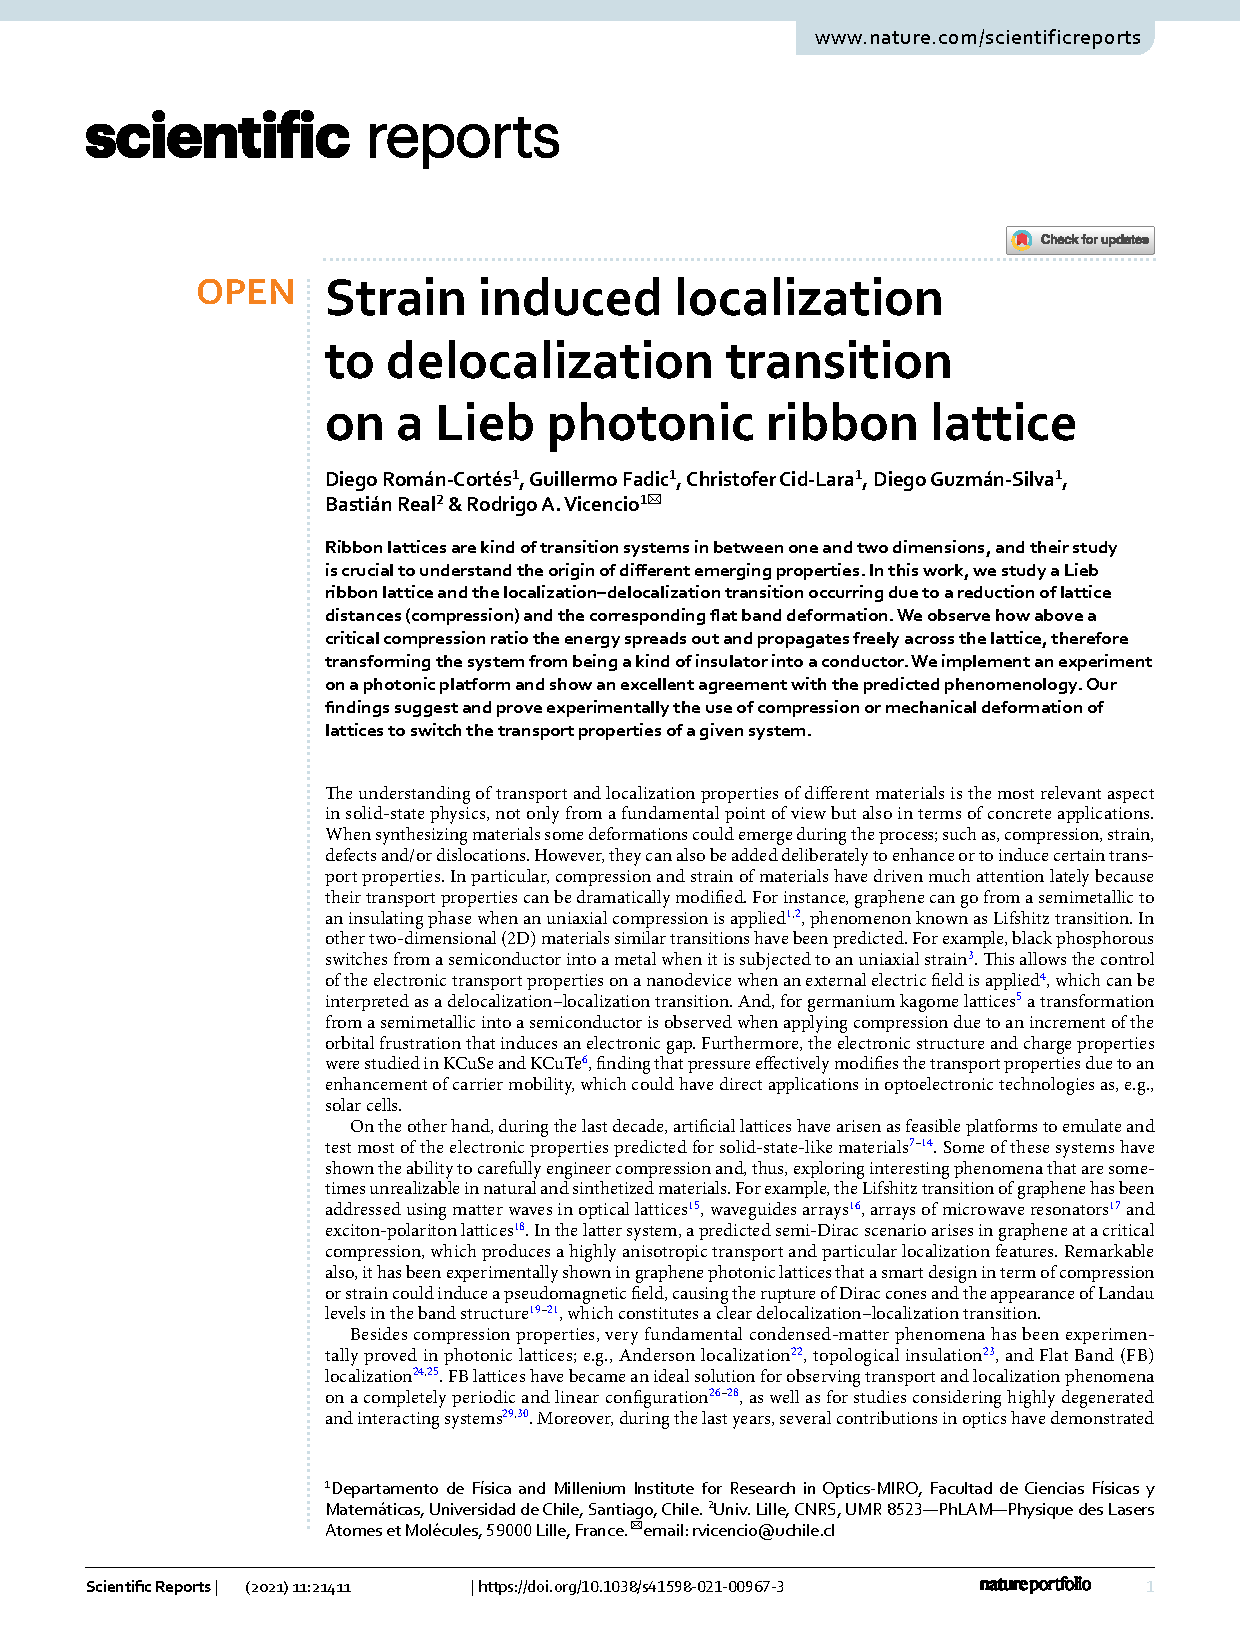
\includegraphics[page=1, width=0.9\linewidth]{media/strainlieb.pdf}
\end{figure}
\newpage
\begin{figure}[H]
	\centering
	\includegraphics[page=1, width=\linewidth]{media/molpap.pdf}
\end{figure}
\newpage
\begin{figure}[H]
	\centering
	\includegraphics[page=1, width=\linewidth]{media/dipolepap.pdf}
\end{figure}
\newpage
\begin{figure}[H]
	\centering
	\includegraphics[page=1, width=\linewidth]{media/nonsympap.pdf}
\end{figure}
\newpage
Aceptado por la revista \textit{Physical Review Letters}, doi:10.1103/b3kw-vv3s:
\begin{figure}[H]
	\centering
	\includegraphics[page=1, width=\linewidth]{media/2Dradpap.pdf}
\end{figure}
\chapter{Condición de ortogonalidad de los modos normales \label{sec:orto}}

La ecuación (\ref{eqn:eigenfield}) permite en encontrar la condición de ortogonalidad de los modos normales del campo eléctrico  $\textbf{E}_k = \textbf{E}_{\perp k}e^{i(\beta_k z - \omega t)}$. Para ello, primero se utilizará el teorema de reciprocidad de Lorentz aplicado a medios dieléctricos. Sean ($\textbf{E}_k$, $\textbf{B}_{k}$) y ($\textbf{E}_{k'}$, $\textbf{B}_{k'}$) soluciones linealmente independientes a las ecuaciones de Maxwell:

\begin{align*}
	\nabla\cdot(\textbf{E}_k\times \textbf{B}_{k'}) &= \textbf{B}_{k'}\cdot(\nabla\times \textbf{E}_k)   - \textbf{E}_k\cdot(\nabla\times\textbf{B}_{k'}) 
\\	
	&= \textbf{B}_{k'}\cdot(i\omega\textbf{B}_{k'})   + \textbf{E}_k\cdot(i\omega n^2/c^2 \textbf{E}_{k'})
	\\
	\implies \nabla\cdot(\textbf{E}_k\times \textbf{B}_{k'} &- \textbf{E}_{k'}\times \textbf{B}_{k}) = 0.
\end{align*}

Haciendo la separación $\nabla = \nabla_\perp + \hat{\textbf{z}}\partial_z$, y notando que $\partial_z (\textbf{E}_k\times \textbf{B}_{k'} - \textbf{E}_{k'}\times \textbf{B}_{k}) =i(\beta_k+\beta_{k'})(\textbf{E}_k\times \textbf{B}_{k'} - \textbf{E}_{k'}\times \textbf{B}_{k}) $
\begin{align}
	\iint_S \nabla\cdot(\textbf{E}_k\times \textbf{B}_{k'} - \textbf{E}_{k'}\times \textbf{B}_{k}) dA
	&= \oint_C (\textbf{E}_k\times \textbf{B}_{k'} - \textbf{E}_{k'}\times \textbf{B}_{k})
	\cdot\hat{\textbf{n}} d\ell \nonumber
	\\
	&=
	- i(\beta_k+\beta_{k'})\hat{\textbf{z}}\cdot\iint_S(\textbf{E}_k\times \textbf{B}_{k'} - \textbf{E}_{k'}\times \textbf{B}_{k})dA \nonumber
	\\
	\implies 
	(\beta_k+\beta_{k'})\int_{-\infty}^{+\infty}\int_{-\infty}^{+\infty}&(\textbf{E}_k\times \textbf{B}_{k'} - \textbf{E}_{k'}\times \textbf{B}_{k})\cdot \hat{\textbf{z}} dxdy = 0, \label{eqn:suma}
\end{align}
pues los campos deben anularse en el infinito. Si consideramos el campo 2 propagándose en la dirección contraria, la ecuación que se satisface es:
\begin{equation}
	(\beta_k-\beta_{k'})\int_{-\infty}^{+\infty}\int_{-\infty}^{+\infty}(-\textbf{E}_k\times \textbf{B}_{k'} - \textbf{E}_{k'}\times \textbf{B}_{k})\cdot \hat{\textbf{z}} dxdy = 0, \label{eqn:resta}
\end{equation}

De (\ref{eqn:suma}) y (\ref{eqn:resta}) se obtiene:

\begin{align}
	 \int_{-\infty}^{+\infty}\int_{-\infty}^{+\infty}(\textbf{E}_k\times \textbf{B}^*_{k'})\cdot \hat{\textbf{z}} dxdy = 0, \text{ si } k\neq k'
\end{align}
\chapter{Código en Python para cálculo de modos normales \label{sec:codigohelmholtz}}

\section{Código en C de BPM \label{sec:codigoBPM}}

\lstinputlisting[language=C]{./codigo/array1d.c}
\chapter{Código en Python generador de hologramas \label{sec:codigoSLM}}

\end{appendices}
\end{document}